
\section{Satellite System Design}
\label{subsec:system-design}
\subsection{Design of the flight and ground segments}
\label{subsubsec:design-flight-ground}
In this subsection, the main characteristics of the system are presented. Objectives, constraints, previous estimations and possible modifications and their effects in the system are exposed.

In a wide vision, it is an \ac{EO} system consisting of a constellation of satellites equally spaced in a \ac{LEO} orbit with the aim of achieving daily coverage of the entire Earth surface. These conditions imply a very sophisticated handle of a huge quantity of data.

The following requirements have been fulfilled to design the system:
\begin{itemize}
\item Swath: $160~km$ (based on state of the art cameras).
\item Resolution: $6.7~m$ (based on state of the art cameras).
\item Low Earth Orbits.
\item Sun Synchronous orbits.
\item Download data rate: $160~Mbps$ (based on Deimos-2 satellite characteristics).
\item Optical Bands: 5 Multispectral (based on state of the art cameras).
\end{itemize}

\paragraph{Global Daily Coverage}~\\
The objective of this system is the acquisition of images of the total Earth surface in a daily basis. Global coverage is considered to include the land surface that is shown in Figure~\ref{fig:intr-land-surface}.


\begin{figure}[!h]
\begin{center}
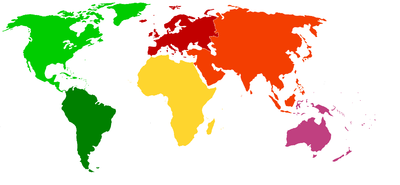
\includegraphics[width=0.6\textwidth]{detaildesign/surface-daily.png}
\caption{Land surface to be acquired in a daily basis}
\label{fig:intr-land-surface}
\end{center}
\end{figure}


\paragraph{Flight Segment}~\\
The satellites are selected according to the current state of the art. However,
some enhancements can be assumed as a way to adjust the analysis to the short
term future.


\subparagraph{Satellite performances}~\\
As a first iteration for the system, small platforms of less of $500~kg$ are
supposed according to the size and payload bay characteristics of representative
platforms in this category. This study is based on the bus platforms currently
offered by Surrey Satellite Technology Ltd, Satrec Initiative and Sierra Nevada Corporation.

In order to reduce the amount of satellites orbiting the Earth, a design with
two payloads was assumed. Thus, the swath (the width of the field of view of each satellite in the surface of the Earth) can be duplicated without decreasing the resolution.

The satellites shall be pointing to nadir, acquiring images without maneuvering
because of the acquisition plan for covering the Earth daily. Simultaneously,
when a satellite gets into the field of view of a Ground Station, the download
of the acquired images starts and at the same time the satellite continues
recording the surface of the Earth.

The main specifications of the satellites in the constellation are shown in Table~\ref{table:intro-satellite-performances}. The values of each parameter were selected according to the state of the art and the desired quality of the images in the mission.

\begin{table}[!h]
  \centering
  {\small
  


\begin{tabular}{p{.2\textwidth}p{.2\textwidth}}
  \tabheadformat
  \tabhead{Specification}   &
  \tabhead{Value}\\
\hline
\textit{GSD}         & $6.7~m$ \\
\hline
\textit{Swath}         & $160~km$ \\
\hline
\textit{Number of bands}         & $5$ \\
\hline
\textit{Digitalization}         & $12~bits$ \\
\hline
\textit{Download Data Rate}         & $160~Mbps$ \\
\hline
\textit{Compression Rate}         &  $2:1$\\
\hline

\end{tabular}


% Local variables:
%   coding: utf-8
%   ispell-local-dictionary: "castellano8"
%   TeX-master: "main.tex"
% End:

  }
  \caption{Main performance parameters of the satellites}
  \label{table:intro-satellite-performances}
\end{table}


\subparagraph{Orbit definition}~\\
The use of \emph{sun-synchronous} orbits in \ac{EO} satellite missions is common. These orbits guarantee that the lighting conditions of the imaged places are the same during the mission, which is a very desirable characteristic.

\ac{LTAN} is also a desired condition of the orbit very related to the lighting
and weather conditions of those places that the satellite overflies (\ac{LTAN}
is selected according to the desired local time of the overflown places and the
cloud formation during the day). The use of \emph{LTAN 10:30h} is commmon for
Earth Observation because at that time the best conditions of cloudiness,
reflectivity and luminosity are given.

Other of the main parameters of an orbit is the altitude. Altitude has effects
in the resolution and the swath of the satellites, which has impact in the
number of satellites required to achieve the coverage objective. According to
the value of those parameters in the payloads included in the satellites, the
reference altitude for the system was found to be $646~km$. \ac{SSO}
condition implies a relation between the altitude and the inclination of the
orbit of $97.97~º$ in this case.

\subparagraph{Number of satellites in the constellation}~\\
The number of satellites is calculated by using the altitude ($646~km$), the
inclination ($97.97~º$) and the swath ($160~km$). As a result, 17 satellites are
required to carry out this mission. In Figure~\ref{fig:intr-constellation-global} the whole constellation is
shown.

\begin{figure}[!h]
\begin{center}
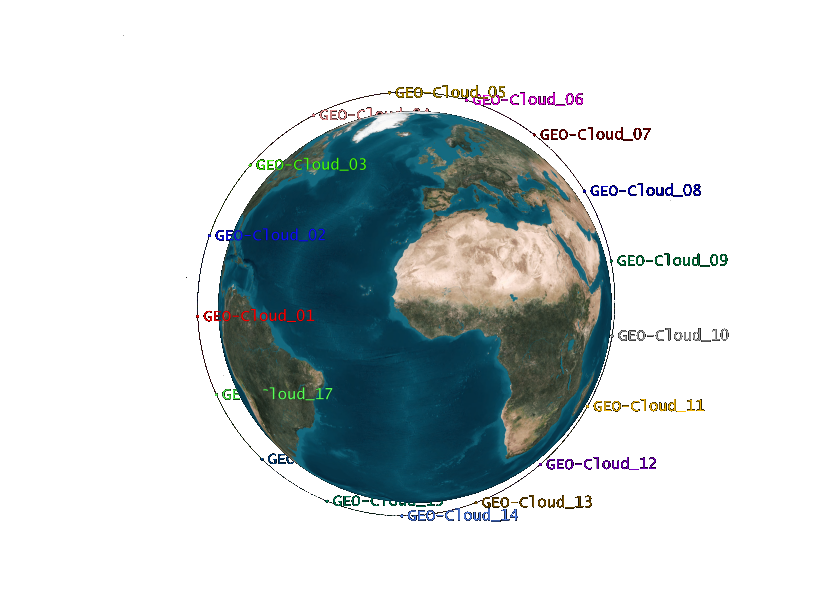
\includegraphics[width=0.75\textwidth]{detaildesign/constellation-global.png}
\caption{Constellation of 17 satellites in a SSO at $646~km$}
\label{fig:intr-constellation-global}
\end{center}
\end{figure}

\paragraph{Ground Stations design}~\\
When the satellite acquires the data, it has to be downloaded to the Ground
Stations. Due to the huge
quantity of data and the limitations to download data rate sets, several
stations distributed over the surface of the Earth are required. They will allow
the satellites to communicate with them and to download the
images. Figure~\ref{fig:intr-footprints} shows how the Ground Stations and their
footprints (area in which the satellites can communicate with the Ground
Station) are distributed.


\begin{figure}[!h]
\begin{center}
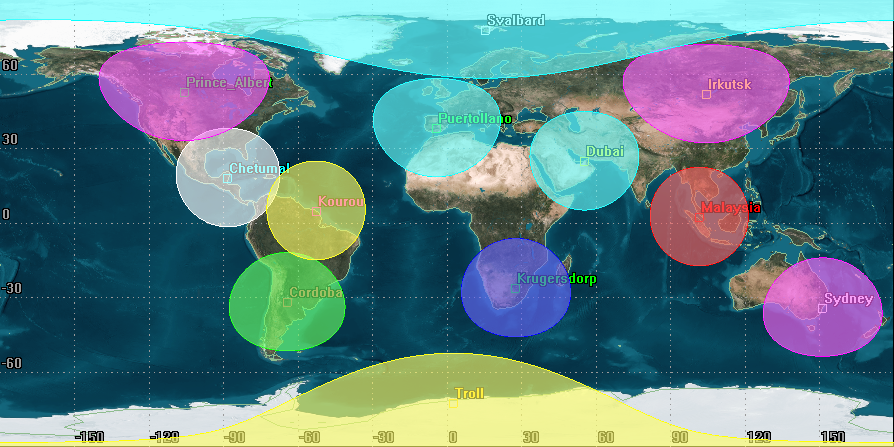
\includegraphics[width=0.85\textwidth]{detaildesign/footprints.png}
\caption{Footprints of the selected Ground Stations}
\label{fig:intr-footprints}
\end{center}
\end{figure}

\subsection{Generated Data Volume}

Specifically, $135,698,500~km^2$ of ground surface are daily acquired. With the
following expression can be estimated the data volume generated:

\begin{equation}
Acquired~Data~Volume= \frac{Acquired~Surface}{GSD^2}~*~Nº bands~*~Digitalization
\end{equation}

Before downloading the images they are compressed. The ancillary data is
included in the process (auxiliary information useful for the geolocation of the
images, satellite status and communication protocol among others). In this case, the ancillary data is estimated to be
12\% of the acquired data (based on Deimos 2 satellite measurements), which is
added and then compressed. With the values depicted in
Table~\ref{table:intro-satellite-performances}, the ancillary and the daily ground
surface adquired, the data on ground can be estimated. As a result, including
ancillary data before compression, $11.55~TBytes$  shall be daily downloaded.

